\section{The Galton--Watson process}
\label{sec:gw}

The Galton--Watson process is the discrete-time, discrete-state branching model in which each individual, independently of every other, is replaced at the next generation by a random number of offspring. Introduced by Galton and Watson in the nineteenth century to study the extinction of family names, it remains the basic object of branching theory \cite{Athreya1972,Harris1963}.

Let the offspring count of a typical individual be the non-negative integer random variable \(\xx\), with
\begin{equation*}
\pr{\xx = k} = p_k,\qquad k = 0,1,2,\dots,
\end{equation*}
and write \(\mu = \mean{\xx}\) for the mean number of offspring. Let \(\zz_n\) denote the size of generation \(n\), starting from a single ancestor \(\zz_0=1\). Conditioning on generation \(n\) and applying the tower property yields
\begin{equation*}
\mean{\zz_{n+1}} = \mean{\mean{\zz_{n+1}\mid \zz_n}} = \mean{\mu\,\zz_n} = \mu\,\mean{\zz_n},
\end{equation*}
hence \(\mean{\zz_n} = \mu^n\). If \(\mu<1\), the expected size decays geometrically and extinction occurs almost surely.

Writing \(\phi(z)=\mean{z^{\xx}}\) for the offspring \pgf{} and \(u_n=\pr{\zz_n=0}\) for the extinction probability by generation \(n\), a first-step argument produces the iteration on which the discrete half of this chapter depends:
\begin{equation}
\label{iterPGF}
u_{n+1} = \phi(u_n).
\end{equation}

\subsection{Death or division}
\label{sec:deathordivision}

Throughout we specialise to the binary (simple) case: each individual either divides into two or dies,
\begin{align*}
p_2 &= p &&\text{(division)},\\
p_0 &= 1-p &&\text{(death)},\\
p_i &= 0 &&\forall\, i\neq 0,2.
\end{align*}
The mean offspring number is then \(\mu=2p\), and the expected size descended from one ancestor is
\begin{equation}
\label{eq:meanZn}
\mean{\zz_n} = (2p)^n.
\end{equation}
The process is subcritical when \(2p<1\), critical when \(p=\tfrac12\), and supercritical when \(2p>1\). \Cref{fig:gwvis} shows genealogical realisations on either side of criticality.

\begin{figure}[ht]
\centering
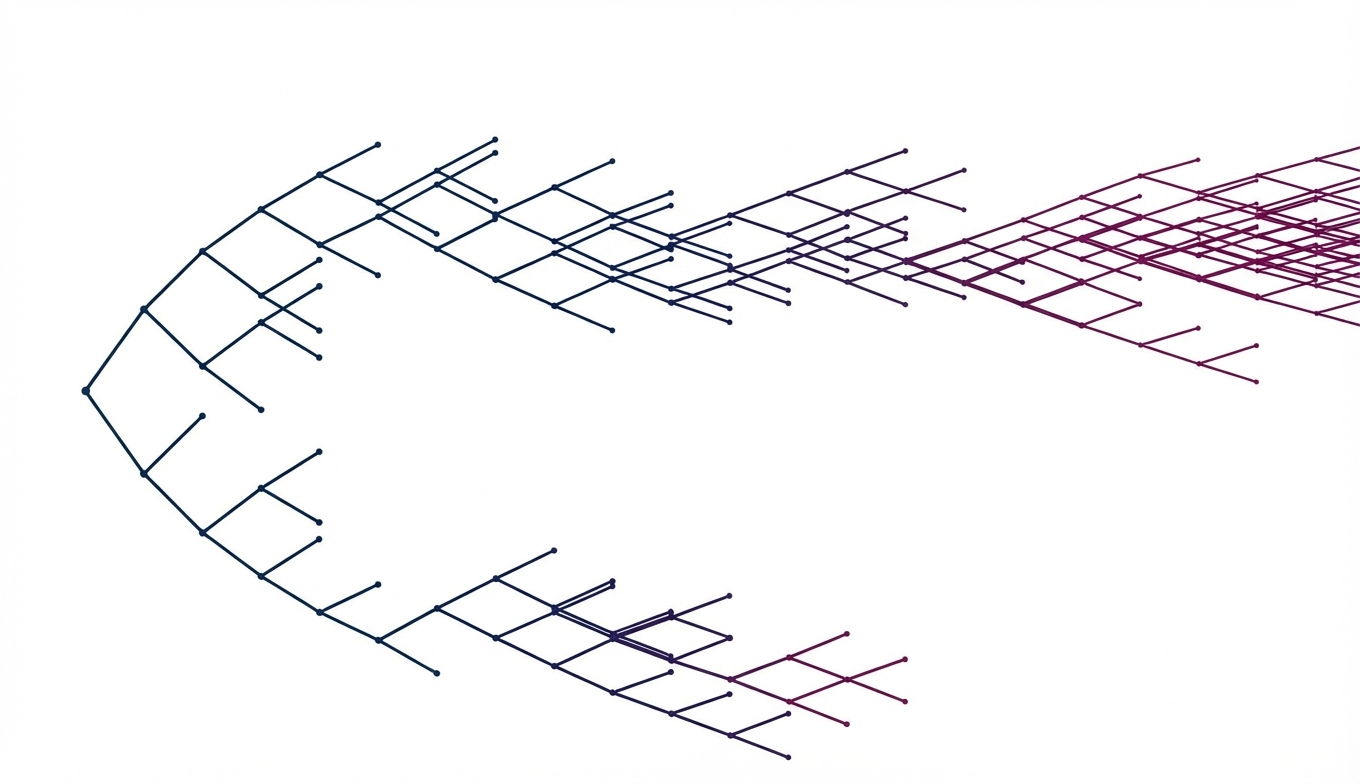
\includegraphics[width=0.78\textwidth]{figures/IMG_ch3/simpleGWvis.png}\\[6pt]
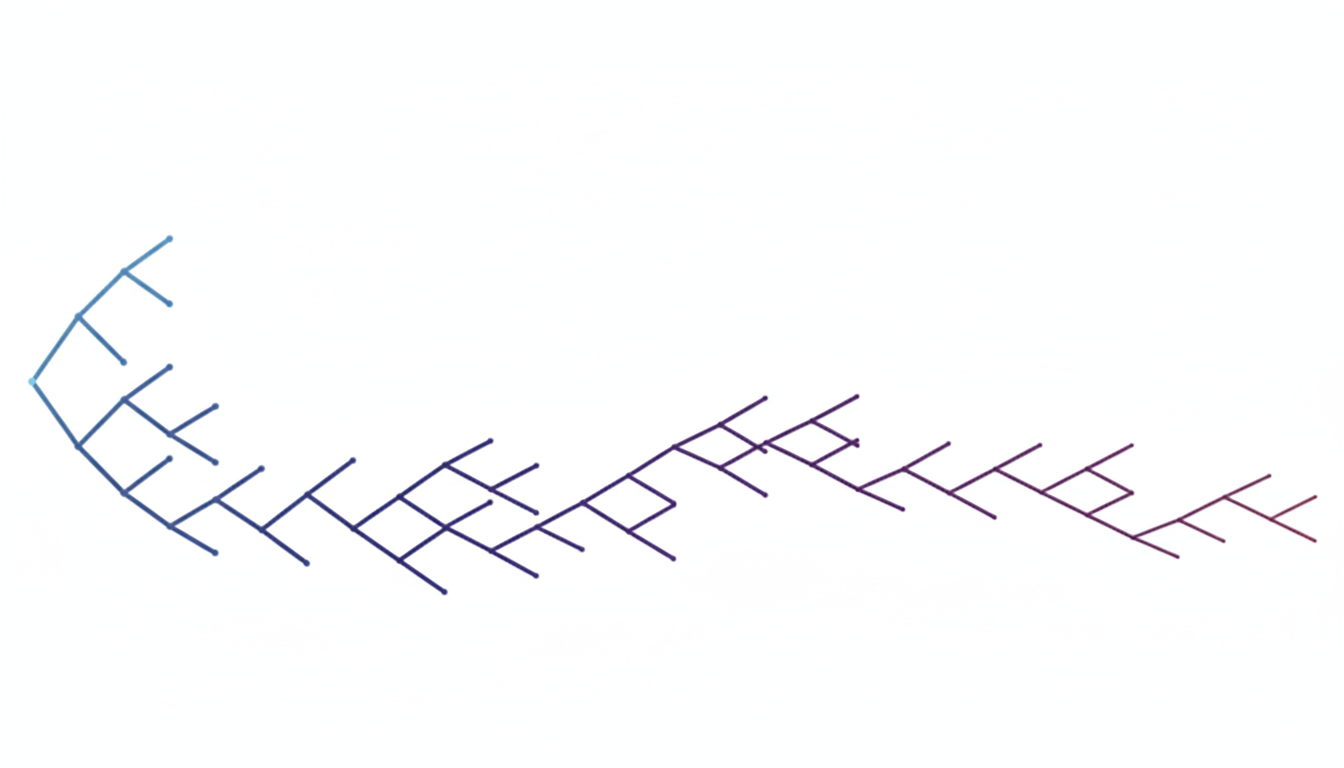
\includegraphics[width=0.78\textwidth]{figures/IMG_ch3/subGWvis.png}
\caption{Realisations of the simple Galton--Watson process, drawn as genealogies with generation increasing to the right. Top: supercritical, \(p=0.58\); the number of lines grows without bound. Bottom: subcritical, \(p=0.47\); the tree terminates. Colour encodes generation number.}
\label{fig:gwvis}
\end{figure}

The offspring \pgf{} is
\begin{equation}
\label{eq:pgfbinary}
\phi(z) = p z^2 + (1-p),
\end{equation}
so that \cref{iterPGF} becomes
\begin{equation}
\label{unIter}
u_{n+1} = p\,u_n^2 + 1-p .
\end{equation}
If the founder dies at the first step (probability \(1-p\)), extinction has already occurred. If it divides (probability \(p\)), extinction by generation \(n+1\) requires each of the two daughter lineages to die out within \(n\) generations, which has probability \(u_n^2\).

It is convenient to work with the survival probability
\begin{equation*}
S_n = 1-u_n = \pr{\zz_n>0}.
\end{equation*}
Substituting \(u_n=1-S_n\) into \cref{unIter} yields
\begin{equation}
\label{SnIter}
S_{n+1} = 2p S_n - p S_n^2,\qquad S_0 = 1.
\end{equation}
Because extinction is irreversible, \(u_n\) is non-decreasing and bounded by \(1\), so \(S_n\) is non-increasing and bounded below by \(0\), and therefore converges to some \(S_\infty\in[0,1]\).

\subsection{Certainty of extinction}
\label{sec:certainty}

Any limit of \cref{SnIter} must be a fixed point. Setting \(S_{n+1}=S_n=S_\infty\),
\begin{equation*}
S_\infty = 2p S_\infty - p S_\infty^2
\qquad\Longleftrightarrow\qquad
p\,S_\infty\bigl(S_\infty + \tfrac1p - 2\bigr) = 0,
\end{equation*}
with roots
\begin{equation*}
S_\infty = 0
\qquad\text{and}\qquad
S_\infty = \frac{2p-1}{p}.
\end{equation*}
For \(p<\tfrac12\) the second root is negative and inadmissible, so \(S_\infty=0\) and extinction is certain. At \(p=\tfrac12\) the roots coincide at the origin and extinction remains certain. For \(p>\tfrac12\) the positive root \(S_\infty=(2p-1)/p\) is attained: survival forever has positive probability. \Cref{fig:phase_transition} displays the transition.

\begin{figure}[htbp]
    \centering
    \begin{subfigure}[b]{0.31\textwidth}
        \centering
        \begin{tikzpicture}
            \begin{axis}[myplotstyle]
                \addplot[blue, thick] {2*0.3*x - 0.3*x^2};
                \addplot[black!45, dashed] {x};
                \addplot[only marks, mark=*, red, mark size=1.6pt] coordinates {(0,0)};
            \end{axis}
        \end{tikzpicture}
        \caption{Subcritical (\(p = 0.3\))}
    \end{subfigure}
    \hfill
    \begin{subfigure}[b]{0.31\textwidth}
        \centering
        \begin{tikzpicture}
            \begin{axis}[myplotstyle]
                \addplot[blue, thick] {2*0.5*x - 0.5*x^2};
                \addplot[black!45, dashed] {x};
                \addplot[only marks, mark=*, red, mark size=1.6pt] coordinates {(0,0)};
            \end{axis}
        \end{tikzpicture}
        \caption{Critical (\(p = 0.5\))}
    \end{subfigure}
    \hfill
    \begin{subfigure}[b]{0.31\textwidth}
        \centering
        \begin{tikzpicture}
            \begin{axis}[myplotstyle]
                \addplot[blue, thick] {2*0.74*x - 0.74*x^2};
                \addplot[black!45, dashed] {x};
                \addplot[only marks, mark=*, red, mark size=1.6pt] coordinates {(0,0) (0.64865,0.64865)};
            \end{axis}
        \end{tikzpicture}
        \caption{Supercritical (\(p = 0.74\))}
    \end{subfigure}

    \vspace{10pt}
    \begin{subfigure}[b]{0.55\textwidth}
    \centering
    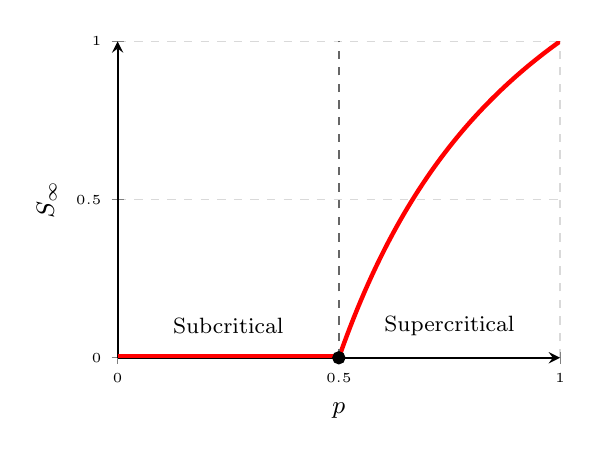
\begin{tikzpicture}
        \begin{axis}[
            width=7.2cm, height=5.6cm,
            axis lines=left,
            xlabel={$p$}, ylabel={$S_\infty$},
            xmin=0, xmax=1, ymin=0, ymax=1,
            xtick={0,0.5,1}, ytick={0,0.5,1},
            grid=major, grid style={dashed, gray!30}, thick,
            label style={font=\small}, tick label style={font=\tiny}
        ]
            \addplot[red, ultra thick, domain=0:0.5] {0.004};
            \addplot[red, ultra thick, domain=0.5:1, samples=120] {(2*x-1)/x};
            \draw[dashed, black!60] (axis cs:0.5,0) -- (axis cs:0.5,1);
            \node[font=\footnotesize] at (axis cs:0.25, 0.10) {Subcritical};
            \node[font=\footnotesize] at (axis cs:0.75, 0.10) {Supercritical};
            \addplot[only marks, mark=*, mark size=2pt, black] coordinates {(0.5,0)};
        \end{axis}
    \end{tikzpicture}
    \caption{The transition in $S_\infty$}
    \end{subfigure}

    \caption{Steady states of the survival recursion \cref{SnIter}. Panels (a)--(c) show the map \(S\mapsto 2pS-pS^{2}\) (blue) against the diagonal (dashed); fixed points are the intersections, marked in red. Below and at criticality the origin is the only fixed point in \([0,1]\), and it is attracting. For \(p>\tfrac12\) a stable positive fixed point \(S_\infty=(2p-1)/p\) separates from the origin, traced in panel~(d).}
    \label{fig:phase_transition}
\end{figure}

\subsection{The critical case: a power law and an infinite expected lifetime}
\label{sec:criticalcase}

At \(p=\tfrac12\) one has \(\mean{\zz_n}=1\) for every \(n\), yet extinction is certain. The reconciliation is that the expected lifetime is infinite: rare trajectories survive for very long times and become very large, at precisely the rate needed to hold the mean at one. The same calculation supplies the asymptotics of \(S_n\) used in \cref{sec:Ap}.

Let \(T=\inf\{n:\zz_n=0\}\) be the extinction time. Writing \(T\) as a sum of indicators and exchanging sum and expectation (all terms non-negative),
\begin{equation}
\label{eq:ETsumSn}
\mean{T} = \sum_{n=0}^{\infty}\pr{T>n} = \sum_{n=0}^{\infty}S_n .
\end{equation}
At \(p=\tfrac12\), \cref{SnIter} becomes \(S_{n+1}=S_n-\tfrac12 S_n^2\), or
\begin{equation*}
S_{n+1}-S_n = -\tfrac12 S_n^2 .
\end{equation*}
For large \(n\) the unit step is small relative to the scale on which \(S_n\) varies, and the left-hand side is well approximated by a derivative:
\begin{equation*}
\frac{\dd S}{\dd n} = -\tfrac12 S^2,
\qquad
S(n) = \frac{2}{n + \text{const}}.
\end{equation*}
Hence
\begin{equation}
\label{twoovrn_sn}
S_n \sim \frac{2}{n}\qquad (n\to\infty),
\end{equation}
confirmed by the simulations of \cref{fig:power_law}(a). Substituting into \cref{eq:ETsumSn}, the tail of the sum behaves like twice the harmonic series and diverges. Thus \(\mean{T}=\infty\): the expected lifetime of the critical process is infinite even though extinction occurs almost surely.

\begin{figure}[H]
    \centering
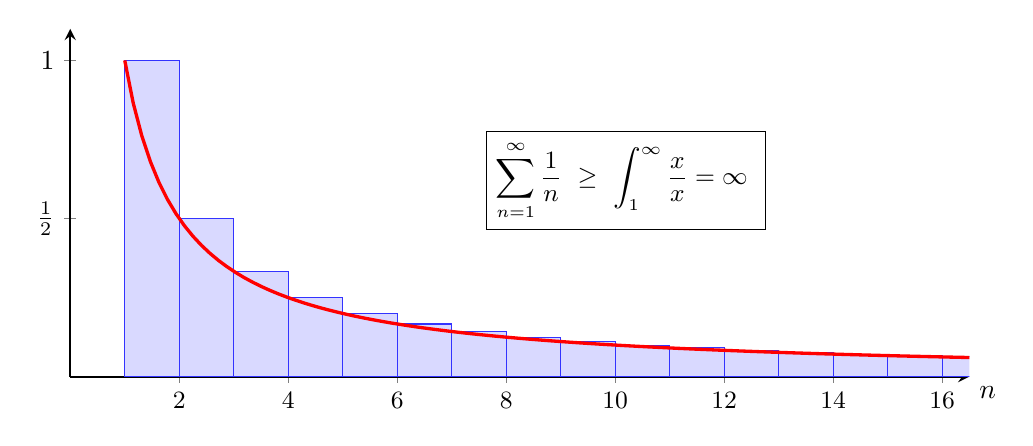
\begin{tikzpicture}
    \begin{axis}[
        axis lines = middle,
        xmin = 0, xmax = 16.5, ymin = 0, ymax = 1.1,
        xlabel = {$n$},
        xtick = {2,4,6,8,10,12,14,16},
        ytick = {0.5, 1}, yticklabels = {$\frac{1}{2}$, $1$},
        axis line style = {thick},
        width = 13cm, height = 6cm,
        every axis x label/.style={at={(current axis.right of origin)}, anchor=north west},
        xticklabel style={font=\small},
    ]
        \addplot[fill=blue!15, draw=blue!80, ybar interval, samples at={1,2,...,17}] {1/x} \closedcycle;
        \addplot[red, domain=1:16.5, samples=100, very thick] {1/x};
        \node[draw, fill=white, align=left, font=\small] at (axis cs: 10.2, 0.62) {
            $\displaystyle \sum_{n=1}^{\infty} \frac{1}{n} \ \ge\ \int_{1}^{\infty} \frac{\dd x}{x} = \infty$
        };
    \end{axis}
\end{tikzpicture}
\caption{Divergence of the harmonic series. Each blue rectangle has area \(1/n\) and contains the region under the curve \(1/x\) on \([n,n+1]\). Because \(S_n\sim 2/n\) at criticality, the same divergence carries over to \(\mean{T}=\sum_n S_n\).}
\label{fig:harmonic}
\end{figure}

\begin{figure}[ht]
    \centering
    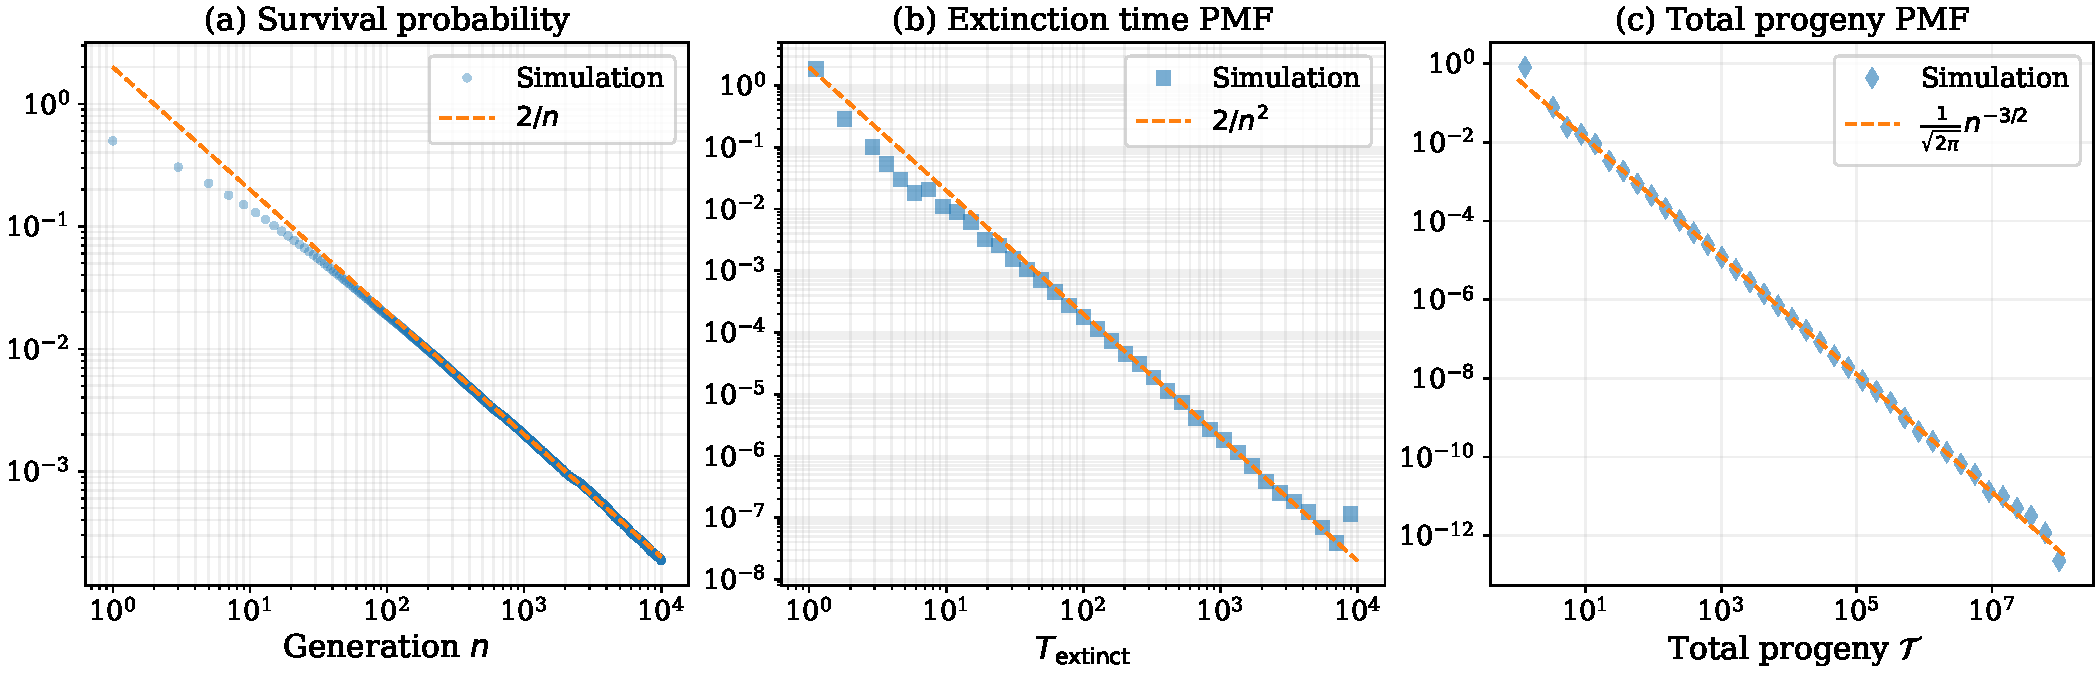
\includegraphics[width=0.98\textwidth]{figures/IMG_ch3/power_law_fixed.pdf}
    \caption{Power-law behaviour in the critical Galton--Watson process (\(p=0.5\)), from \(10^6\) realisations.
    (a) Survival probability \(S_n=\pr{\zz_n>0}\), showing \(S_n \sim 2/n\).
    (b) Probability mass function of the extinction time \(T\), with heavy tail \(\pr{T = n}\sim 2/n^{2}\).
    (c) Probability mass function of the total progeny \(\mathcal{T} = \sum_{k\ge0}\zz_k\), with the classical critical asymptotic \(\pr{\mathcal{T}=n}\sim n^{-3/2}\).}
    \label{fig:power_law}
\end{figure}

\FloatBarrier
